% !TEX TS-program = pdflatex
% !TEX encoding = UTF-8 Unicode

% This is a simple template for a LaTeX document using the "article" class.
% See "book", "report", "letter" for other types of document.

\documentclass[11pt]{article} % use larger type; default would be 10pt

\usepackage[utf8]{inputenc} % set input encoding (not needed with XeLaTeX)

%%% PAGE DIMENSIONS
\usepackage{geometry} % to change the page dimensions
\geometry{a4paper} % or letterpaper (US) or a5paper or....
% \geometry{margin=2in} % for example, change the margins to 2 inches all round
% \geometry{landscape} % set up the page for landscape
%   read geometry.pdf for detailed page layout information

\usepackage{graphicx} % support the \includegraphics command and options

% \usepackage[parfill]{parskip} % Activate to begin paragraphs with an empty line rather than an indent

%%% PACKAGES
\usepackage{booktabs} % for much better looking tables
\usepackage{array} % for better arrays (eg matrices) in maths
\usepackage{paralist} % very flexible & customisable lists (eg. enumerate/itemize, etc.)
\usepackage{verbatim} % adds environment for commenting out blocks of text & for better verbatim
\usepackage{subfig} % make it possible to include more than one captioned figure/table in a single float
% These packages are all incorporated in the memoir class to one degree or another...

%%% HEADERS & FOOTERS
% \usepackage{fancyhdr} % This should be set AFTER setting up the page geometry
% \pagestyle{fancy} % options: empty , plain , fancy
% \renewcommand{\headrulewidth}{0pt} % customise the layout...
% \lhead{}\chead{}\rhead{}
% \lfoot{}\cfoot{\thepage}\rfoot{}

%%% SECTION TITLE APPEARANCE
\usepackage{sectsty}
\allsectionsfont{\sffamily\mdseries\upshape} % (See the fntguide.pdf for font help)
% (This matches ConTeXt defaults)

%%% ToC (table of contents) APPEARANCE
\usepackage[nottoc,notlof,notlot]{tocbibind} % Put the bibliography in the ToC
\usepackage[titles,subfigure]{tocloft} % Alter the style of the Table of Contents
\renewcommand{\cftsecfont}{\rmfamily\mdseries\upshape}
\renewcommand{\cftsecpagefont}{\rmfamily\mdseries\upshape} % No bold!

% Package to insert code
\usepackage{xcolor}
\usepackage{listings}
\lstset{language=[ISO]C++}	%set code language
\lstset{basicstyle=\small\ttfamily,
		keywordstyle = \color{blue}\bfseries,
		commentstyle = \color{gray},
		stringstyle = \color{green}}	% code style
\lstset{tabsize=2}	% tabulation for code
\lstset{backgroundcolor = \color{yellow!7}}
\newcommand{\classname}[1]{\texttt{#1}}

% Maths packages
\usepackage{amssymb}
\usepackage{amsmath}

% Bellezza documento
\usepackage{microtype}

% Package for smaller captions
\usepackage[font=small]{caption}


%%% END Article customizations

%%% The "real" document content comes below...

\title{BGLgeom library}
\author{Speranza Ilaria (matr. 854196) \\ Tantardini Mattia (matr. 858603)}
%\date{} % Activate to display a given date or no date (if empty),
         % otherwise the current date is printed 

\begin{document}
\maketitle
\newpage
\tableofcontents
\newpage

\section{Introduction}
	The purpose of the project is to extend the Boost Graph Library (BGL) providing it more functionalities and making it capable to handle graphs with geometric properties, that the BGL currently does not support. This mainly means to provide a graph from BGL, that already implements all topological operations, a way to describe its vertices as points and its edges as generic curves in the space (2 or 3 dimensional). Moreover, classes which implement these kind of geometrical properties must be able to carry out geometric and analytic operations, such as computation of first and second derivative of the curves describing edges and creation of numerical meshes on them. \newline
	All the geometric functionalities we developed in the library are aimed at solving numerical problems which can be modelled using a graph, but which also are in a geometric setting or need it: for instance, to compute flows in a network of blood vessels, meshes are required to solve finite element problems, and so it can be very useful to couple the graph description with the geometric one. \newline
	A lot of different kind of applications can take advantage from this library; in particular, we provide two example of specific applications: one that creates a graph computing intersection of fractures in a fractured porous media, and the other that solves a simple diffusion problem on a vascular network.

\section{The library}
	\subsection{Briefs on BGL}
	The BGL is a template library to create, handle and operate on graphs. It implements some different classes of graphs, all the topological operations concerning them, and a wide variety algorithms.
	\newline\newline
	% Metto qui quello che ho messo nella documentazione? adjacency_list e tutto il resto? forse comunque ho bisogno di dire dell'adjacency list, ma
	Among all these functionalities, we decided to focus on a single class to describe a graph and on how implement in an easy to use way the geometrical properties. To explain in more details our implementation choices, we need to spend some words on how that class and the graph properties work.
	
		\subsubsection{The adjacency\_list class}
		\classname{adjacency\_list} is a template class which represents a graph with a two dimensional structure: 
		a \texttt{VertexList} and a \texttt{OutEdgeList} container. The first one stores all the vertices of the graph, and each vertex contains the other one-dimensional structure which is the list of all the out-edges leaving that vertex (so only out-edges if the graph is directed, all the edges if the graph is undirected). \newline
		The class has five template parameters and the full protoytpe is: \classname{adjacency\_list< OutEdgeList, VertexList, Directed, VertexProperties, EdgeProperties >}. \newline
		The first two template parameters allow to choose the types of the underlying containers for the bidimensional structure. Choosing them affects space complexity of the graph and efficiency of some operations, such as inserting and removing edges. In our work we always set them to the selector \classname{boost::vecS} (that stands for \texttt{std::vector}) for ease of use and since, from BGL documentation, it is on average the best performing choice for every topological operation. \newline
		The third template parameter obviously allows to choose between a directed or undirected graph.\newline
		The last two template parameters are the most interesting ones: they allow to choose what are the vertex and the edge properties. The BGL provides an easy way to handle them: the so called \textit{bundled properties}. They simply are classes, or better, structs, which can be passed as template parameter to the \classname{adjacency\_list} class, and they will become its vertex and edge properties, along with all their attributes and memeber functions. This gives a lot of flexibility: for instance, if we want all the vertices to have as properties three doubles, an int, two strings and a member that returns a random number, we only have to define them all in the same struct and pass it as the fourth template parameter of the \classname{adjacency\_list} class. The same for the edges, passing the corresponding struct as fifth template parameter. Moreover, the usage of a struct, instead of a class, enables public member access, and this comes out in a slight more ease of use when accessing the properties. \newline
		Concluding this description, we underline that choosing different values for the template parameters consits in changing the type of the graph one is using, with consequence on some other tool provided by BGL.
		
		\subsubsection{Vertex and edge descriptors}
		Two specific handles are provided to manipulate vertices and edges: the vertex and the edge descriptors. They may be of different types, depending on the graph type. They in general 'refer' to a particular vertex or edge, thus allowing for instance to access their properties, or to specify in a very readable way topological operations. \newline
		Two more tools are provided to access a graph: vertex and edge iterators. As the descriptors, the iterators can be of different types depending on the graph type. Specific function return the iterator to the first and last vertex and to the first and last edge in the graph, thus allowing graph traversal. Dereferencing an iterator, the descriptor of the vertex or edge pointed by that iterator are obtained. \newline
		Both descriptors and iterators are accessible through the \classname{graph\_traits} class.
		
		\subsubsection{Accessing properties}
		Using \textit{bundled properties}, BGL provides an easy way to acces vertex or edge properties: just use the \texttt{operator[]} on a graph object, with index the descriptor of the vertex or edge whose properties one wants; this will consists in accessing the struct used as vertex or edge property. Since a struct has public access, with the dot operator we can immediately read from or write in each attribute or call a member function.
		
		% Mettere del codice di esempio qui????
	
	
	\subsection{BGLgeom}
	This is the library we developed to meet the goals of the project. The name is the union of "BGL", since this wants to be an extension of it, and of "geom", that stands for "geometry", to indicate the aim of the main functionalities added. 
	\newline\newline
	The library comes from the need to have a common environment where to build and run very different types of applications, but with a geometrical setting and an underlying graph structure in common. This implies, besides the development of the geometric properties, the implementation of input/output utilities, to make this library produce useful outputs for other softwares. From this point of view, this library can be a common starting point for different projects and applications.
	\newline\newline	
	%We build a template library capable to handle 2 and 3 dimensional geometries. Most geometric characteristics, such as points, geometries for the edges, etc, are templatized on the dimension of the space. Another recurrent template parameter is the type of the graph used, needed in most cases to use the tools from BGL. 
	
		\subsubsection{What is inside}
		The library contains many things:
		\begin{itemize}
			\item \textbf{Adapters for BGL}: we provide some layers and additional functions to hidden the most used native BGL ones and to improve readibility and ease of use.
			\item \textbf{Classes to build graph properties}: the main part of the library are all the classes we developed to create a vertex and an edge property including the basic geometric requirements.
			\item \textbf{Geometrical and numerical utilities}: we included in this library some code to compute integrals, generate meshes, compute intersections between linear edges.
			\item \textbf{I/O utilities}: we provide one reader class to read tabular ASCII files, and three writer classes to produce three different types of output: ASCII, .pts and .vtp files.
			\item \textbf{Tests}: we provide source code examples to show how the main classes and writers work.
		\end{itemize}
	
		%forse posso dire prima quali proprietà geometriche abbiamo implemenmtato, come e perché, e poi come le abbiamo messe insieme per poter usare i grafi.
	
		\subsubsection{Geometric properties}
		In this library we do not provide any type of grap. We decided to use the \classname{adjacency\_list} class directly from the BGL, since this already gives a lot of flexibility. We focused on implementing the geometrical properties we were required as \textit{bundled properties} (that are really flexible too), so that we could simply pass them as template parameters to create a graph with the desired characteristics. Moreover, we chose to put in our properties only the functionalities that are really needed for a geometrical description, leaving the user the freedom to add its own characteristics and functionalities. \newline
		The geometric properties we were asked to developed are:
		\begin{itemize}
			\item Coordinates for points.
			\item Boundary conditions.
			\item Parameterization for the edges, along with computation of the main characteristics: first and second derivative, curvature, curvilinear abscissa.
			\item Meshes on the edges.
		\end{itemize}
		We templated all this elements on the dimension of the space.				
		\paragraph{Points.}	To represent points we used \texttt{Eigen} matrices, with 1 column and n rows. We choose the \texttt{Eigen} because it provides high efficiency and a lot of numerical methods to compute in an easy way geometrical quantities.
		\paragraph{Boundary conditions.} We implemented a class to store a boundary condition as a type and a value. We provided an \texttt{enum class BC\_type} to represent the most common types of boundary conditions.
		\paragraph{Edge geometries.} Concerning the geometry and parameterization of the edges, we were asked to be as generic as possible, that is the library should have been able to manage any possible parameterization of the type
		\begin{equation*}
			f:\mathbb{R}\rightarrow\mathbb{R}^{n} \quad, \quad n=2,3 ,
		\end{equation*}
		i.e. from a line to a generic curve in the plane or in the space. We met this goal by developing three different classes: the \classname{linear\_geometry} class for the straight lines, and the \classname{generic\_geometry} and \classname{bspline\_geometry} classes for a generic curve.
%		\newline
%		All this classes hold a parameterization of the curve inbetween 0 and 1, so we actually have parameterizations of the type
%		\begin{equation*}
%			f:[0,1]\rightarrow\mathbb{R}^{n} \quad, \quad n=2,3.
%		\end{equation*}
%		for each geometry. All classes derive from an abstract class, \classname{edge\_geometry}, which specifies the functionalities that the geometry of an edge should have: in our case, they are the evaluation of the curve, the computation of first and second derivative, curvature and curvilinear abscissa at given value (or a vector of values) of the parameter.
		%Descrizione di ogni geometry?
		\paragraph{Meshes.} We provide a class that is at the same time a mesh generator and a container for two type of meshes: the parametric one, generated from the parameterization of the edge, and the real one, that is the evaluation of the parametric mesh on the same edge. We decided to keep also the parametric mesh since it may be useful to evaluate it to get also other quantities, such as curvature, in correspondence of the points of the real mesh.
		
		\subsubsection{Edge geometries}
		All geometry classes derive from an abstract class, \classname{edge\_geometry}, which specifies the functionalities that the geometry of an edge should have: in our case, they are the evaluation of the curve, the computation of first and second derivative, curvature and curvilinear abscissa at given value (or a vector of values) of the parameter. All the classes hold a parameterization of the curve inbetween 0 and 1, so we actually have parameterizations of the type
		\begin{equation*}
			f:[0,1]\rightarrow\mathbb{R}^{n} \quad, \quad n=2,3.
		\end{equation*}
		for each geometry. We made this choice to adopt a common interface for the three geometries; all classes performs controls on the value of the parameter: if it is out of bounds, the class will show an error message and stop the execution. All the three classes are templatized on the dimension of the space.
		\paragraph{Linear geometry.} The \classname{linear\_geometrye} class obviously describes straight lines. It stores as internal attributes the coordinates of the source and the target of the edge it describes. This may be memory inefficient in large graphs, since the information about the coordinates are already stored in the vertices, but otherwise it would have required a lot of operations and to build a more complex structure to recover those information. In this way we give directly access inside the class. The coordinates of source and vertex are used to rescale the parameterization from [0,1] to the real position in the space. It is a very efficient class, since it performs only simple algebraic operations to compute evaluation, first derivative and curvilinear abscissa, and returns directly zero for the second derivative and the curvature.
		\paragraph{Generic geometry.} The \classname{generic\_geometry} class can store the exact parameterization of any curve. We implemented it using the \texttt{std::function} wrapper, and it requires to provide the exact analytic expression of the curve and of its first and second derivative, each one parametrized between 0 and 1 (it is care of the user to do this). The evaluation members just evaluate the functions stored in the private attributes.
		\paragraph{Bspline geometry.} The \classname{bspline\_geometry} class stores a description of the curve as a bspline. To build this representation, at least vector of control points is required. The class is thus able to store any curve, giving it all the analytic properties of the bspline curves. This class stores as private attributes the control points for the curve, for its first and second derivatives (that are bsplines as well by property); this implies that the class is more memory consumptive. To evaluate the curve and the derivatives, the class performs some more computation than in the other classes.
		
		\subsubsection{Building a geometric graph}		
		\paragraph{The geometric base properties.} We developed the structs \classname{Vertex\_base\_property} and \classname{Edge\_base\_property}, that are thought to be the base vertex and edge property for a graph which wants to have a geometric description. They are substantially two containers, which gather the previous described classes.
		In the \classname{Vertex\_base\_property} we included:
		\begin{itemize}
			\item The coordinates of the point in the space representing the vertex.
			\item A \texttt{std::array} to store the boundary conditions on that vertex. We templatized the array on the number of the boundary conditions the user wants, since it may happen for some applications that more than one FEM problem has to be solved on the graph, thus requiring more than one boundary condition for each vertex.
		\end{itemize}
		In the \classname{Edge\_base\_property} we included:
		\begin{itemize}
			\item One among th three geometry class.
			\item A mesh class.
		\end{itemize}
		The \classname{Edge\_base\_property} is templated on the edge geometry one wants.
		Both properties are also provided with two more attributes: an index and a label. These may be useful to give to vertices and edges a specific ordering and to keep track of and reconnaise particular parts of the graph.
		\paragraph{A first Example.} To create a geometric graph with the above properties, we now only have to declare an object of class \classname{adjacency\_list} with \classname{Vertex\_base\_property} as fourth template parameter and with \classname{Edge\_base\_property} as fifth template parameter. For instance:
\begin{lstlisting}[frame=single]
using Edge_prop = 
	BGLgeom::Edge_base_property< BGLgeom::linear_geometry<3>, 3 >;
using Vertex_prop = BGLgeom::Vertex_base_property<3>;
using Graph = 
	boost::adjacency_list< boost::vecS, boost::vecS, 
		boost::directedS, Vertex_prop, Edge_prop >;
Graph G;
\end{lstlisting}
		Note that the we created and empty graph and that all the properties, especially geometries for edges, have to be set up with all the needed values while building the graph. Moreover, note that, since the chosen geometry for the edge properties \texttt{Edge\_prop } is \texttt{linear\_geometry}, and since this \texttt{Edge\_prop} is passed as template argument to the \classname{adjacency\_list} class, the whole graph will have edges with linear geometry. \textit{This is a kind of 'static' property of the graph. A future development of the library may consider to create a kind of 'dynamic' \texttt{Edge\_base\_property}, that is capable to hanlde different geometries on different edges.} %Maybe lo possiamo mettere nei todo's questo. 
		\paragraph{Extending base properties.} We created our first new geometric graph with the properties provided by our library. But in the applications a lot of other quantities and parameters may be necessary, for instance diameter and pressure for a blood vessel, or permeability for fractures, or any other kind of variable. How to expand the basic geometric properties of vertices and edges we provide to contain the new variables? Just publicly inherit from our base properties, and define at least a default constructor. This is not mandatory unless you use pointers in your derived properties, but we strongly suggest to implement it to prevent bad behaviours. A generic example is:
\begin{lstlisting}[frame=single]
struct My_vertex_prop : public BGLgeom::Vertex_base_property<3> {
	double variable1;			// may be pressure
	int varaible2;				// some flag
	std::string a_string;	// a description
	my_class object;			// may be solver for FEM problem on edge
	
	My_vertex_prop() : BGLgeom::Vertex_base_property<3>(),
										variable1(.0),
										variable2(0),
										a_string(),
										object() {};	
};
\end{lstlisting}
		The use of inheritance is a fast way to derive your own vertex or edge property with a lot of freedom, and also allows access in a fast and easy way to the inherited geometric properties.
		\paragraph{Adding vertices and edges.} To add new edges and vertices to a graph the user substanqially uses the already existent \texttt{boost} functions which make that job. We only hid them under external functions which recall the name: \texttt{BGLgeom::new\_vertex} and \texttt{BGLgeom::new\_edge} instead of \texttt{boost::add\_vertex} of \texttt{boost::add\_edge}. We provided different overloads: just adding vertex and edge, adding them along with their properties, performing additional checks on the insertion of the edges. Furthermore, we added three new functions (\texttt{BGLgeom::new\_linear\_edge}, \texttt{BGLgeom::new\_generic\_edge} and \texttt{BGLgeom::new\_bspline\_edge}) to add edges, to provide an easy way to add a new edge to the graph already with its geometry set up in the proper way.	On how to use the functionality we provided to build a graph, see the source code \textit{test\_BGL\_vs\_BGLgeom.cpp}.
			
		\subsubsection{Reader class}		
		We provided in this library a generic ASCII reader to read topology and properties of the graph from a tabular file. The reader is a tempalte abstract class. It is templatized on the vertex and edge properties of the graph, thus making the same reader suitable for every kind of vertex and edge property a graph will have. There is a third template parameter, defaulted to an empty struct type, that represents the topological information one wants to read about the graph; they may not be needed, since they can be omitted in particular formats of file (for instance, specifying coordinates of source and target of an edge already tells us the topology; while if indexes for vertices and edges are provided, the topology can be handled in an easier way). \newline
		We left as pure virtual the members those devoted to read data from file and to return the just read data as vertex or edge properties. While deriving his own concrete reader, the user has to specify:
		\begin{itemize}
			\item all the variable members needed to store the read data;
			\item how to read (in the right order) from the file the data for each single edge, using the inner stream attribute, in the member \texttt{get\_data()};
			\item how to pack the data read into a vertex property which will be assign to the source and target of the edge he is reading in the members \texttt{get\_source\_data()} and \texttt{get\_target\_data()};
			\item how to pack the data read into the edge property which will be assigned to the new edge in the member \texttt{get\_edge\_data()};
			\item if topological information are provided, how to pack them in a struct that will contain this kind of information, otherwise he has to define the \texttt{get\_topological\_data()} as a member that returns an empty struct (however in this case it won't be used).
		\end{itemize}
		Note that the reader is thought to read one edge at a time from the file and to return the vertex and edge properties related to the edge just read and to its source and target. In this way, it is easy to build a graph in a loop, reading one edge at a time from the file, adding it to the graph and immediately update its properties (and the properties of its source and vertex), before reading and adding a new edge. \textsl{The only drawback of this strategy is some lack of efficiency concerning the vertex properties: it may happen that new edges coming in the graph will have as source and target already existing vertices, and thus the algorithm will update more than once their properties. If the graph has high average rank, this drawback may be solved performing a check whether the source and the target for an incoming edge already exist in the graph, or by keeping track in some way of the vertex descriptor of the vertices already inserted}. \newline
		As final observation, we remember that the reader is able to read all kind of tabular file which have as delimiter among the various columns spaces or tabulations, but not commas (unless they are read as more data that will be discarded).
		
		\subsubsection{Writer classes}
		Three kind of writers are provided to output the graph and its properties; each one produce a different format of output.
		\paragraph{Writer\_ASCII.} The \texttt{writer\_ASCII} class produces as output a tabular format (.txt, .dat, etc). It is an abstract class with about the same philosophy of the \texttt{reader\_ASCII} class: the user has to define its concrete writer, telling him which properties of the graph to print, and how. The pure virtual member devoted to this is \texttt{write\_data}, which wants as arguments the graph and the edge descriptor of the edge we want to printo information about. Remember that from an edge descriptor one is always able to recover the source and target properties through their vertex descriptors, using the \texttt{BGLgeom::source()} and \texttt{BGLgeom::target()} functions. Also in this case, it will easy to print information about the graph in a loop over all the edges.
		\paragraph{Writer\_pts.} The \texttt{writer\_pts} class produces a particular kind of output (.pts), with a particular format: it express the graph as a sequence of arcs, and for each arc are printed the boundary conditions on source and target and all point of the mesh defined on it (if present, otherwise only source and target coordinates) are printed. We developed such a writer since we use the GetFem++ library in the application on diffusion in a vascular network, and the .pts format is the input one for Getfem to read meshes, and then solve FEM problems. \newline
		To meet some requests from people that will use our library with the GetFem one for further applications, we also developed some particular features for the writer. We provided it with an additional template parameter, the number of boundary conditions (defaulted to one): if specified different from 1, it will produce different output files, each one with the same structure but with different boundary conditions. Another feature allows to print in a separate file some geometric information (first and second derivative, curvature) in correspondence of the points of the mesh (if present) on each edge.
		\paragraph{Writer\_vtp.} The \texttt{writer\_vtp} class produces a .vtp output, i.e. a VTK polygonal data format. It is a particular format provided by the wider VTK library. It consist in an XML file in which all the topology of the graph is coded. The output consists into two file: one coding the edges, and one coding the vertices of the graph. This kind of output is thought to visualization purpouse: using for instance software such as Paraview, the output files can be easily displayed, giving a visual representation of the graph, to which the visualization of other quantities significant for the application can be added.
	
		\subsubsection{Todos}
		\paragraph{Edge base property.} The \classname{Edge\_base\_property} we provide in the library is a kind of 'static' one: it contains one of the three geometries, and the type is chosen passing it through a template parameter. And then the \classname{Edge\_base\_property} itself is passed as template parameter to create the graph. This implies that the geometry of all the edge in the graph will be fixed to the one used as template parameter. This behaviour may be inefficient for some applications, for instance when the underlying graph has almost all linear edges and only few edges that would be better to model with a curve geometry. At this stage, the geometry of such a graph will be fixed to the generic or bspline one for all edges, thus giving some memory and computational inefficiency on the edges that could have been described by the linear geometry. For this reason, it may be interesting from an efficiency point of view to implement a kind of 'dynamic' version of the \classname{Edge\_base\_property}, to make the user be able to select a different geometry for each different edge in the graph.

\section{Applications}
	In this section we present two examples from real situations, using tools from BGLgeom library to model and solve them.

	\subsection{Fracture Intersection}
%		\subsubsection{The problem}
	In this example a list of fractures, all lying on the same plane, is given as input. The goal is to build a graph representing the network, with vertices in correspondence of the fractures' extremities and of the intersection points  and edges representing the fractures. A very simple example is shown in figure \ref{fig:frac_int_example}.
	\begin{figure}
		\centering 
		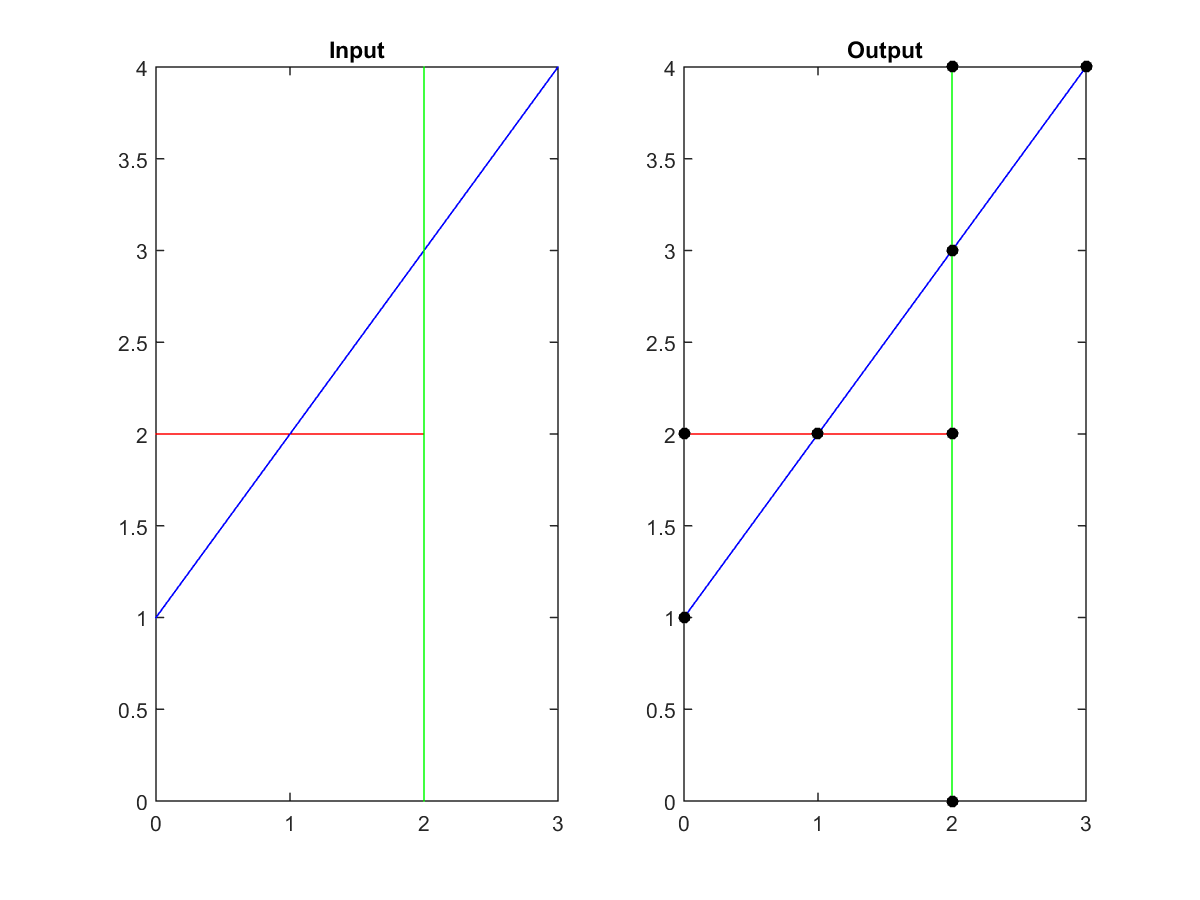
\includegraphics[width=0.5\textwidth]{frac_inters}
		\caption{Example}
		\label{fig:frac_int_example}
	\end{figure}
	
		\subsubsection{Intersection types}
		To compute the intersection between two given edges we used a piece of code, developed by Professor Formaggia, which we included as a utility in our libary BGLgeom (\texttt{intersections2D.hpp}), after adapting it to our specific data structeres, as a struct, \texttt{Intersection}: it stores the number of intersections, the intersection point (if the intersection is not just a point but a segment, its two extremes are returned), two boolean variables, whose value depend respectively on the parallelism and the collinearity of the evaluated edges, and the intersection type.\newline
		The intersection type is an enum class with 12 different values, 10 corresponding to real intersections and listed in figure \ref{fig:frac_int_type}, plus two handling the case with no intersection and the case of some unexpected behaviour.
		Depending on the intersection type, different actions will be performed during the graph construction.
		For this specific application we also created in file \texttt{fraxture\textunderscore intersection/include/intersections2D\textunderscore utilities.hpp} a struct called \texttt{Int\textunderscore layer}, whose constructor takes as input an \texttt{Intersection} struct and computes from it variables of interest:
		\begin{itemize}
			\item how: intersection type, directly copied from \texttt{Intersection}
			\item int\textunderscore edge: edge descriptor of the intersected edge
			\item int\textunderscore pts: intersection point(s), directly copied from \texttt{Intersection}
			\item swapped\textunderscore comp: boolean equal to 1 when there are two intersection points and they are swapped while ordering the intersection vector
			\item intersected\textunderscore extreme\textunderscore old: boolean equal to 0 if the source of the "old" edge (that already in the graph) is an intersection point, equal to 1 if the target of the "old" edge is involved. This variable is used only when we already know from the intersection type that one and only one extremity of the "old" edge is an intersection point.
			\item intersected\textunderscore extreme\textunderscore new: boolean equal to 0 if the source of the "new" edge (the fracture currently added) is an intersection point, equal to 1 if the target of the "new" edge is involved. This variable is used only when we already know from the intersection type that one and only one extremity of the "new" edge is an intersection point.
		\end{itemize}
		
		\begin{figure}
			\centering 
			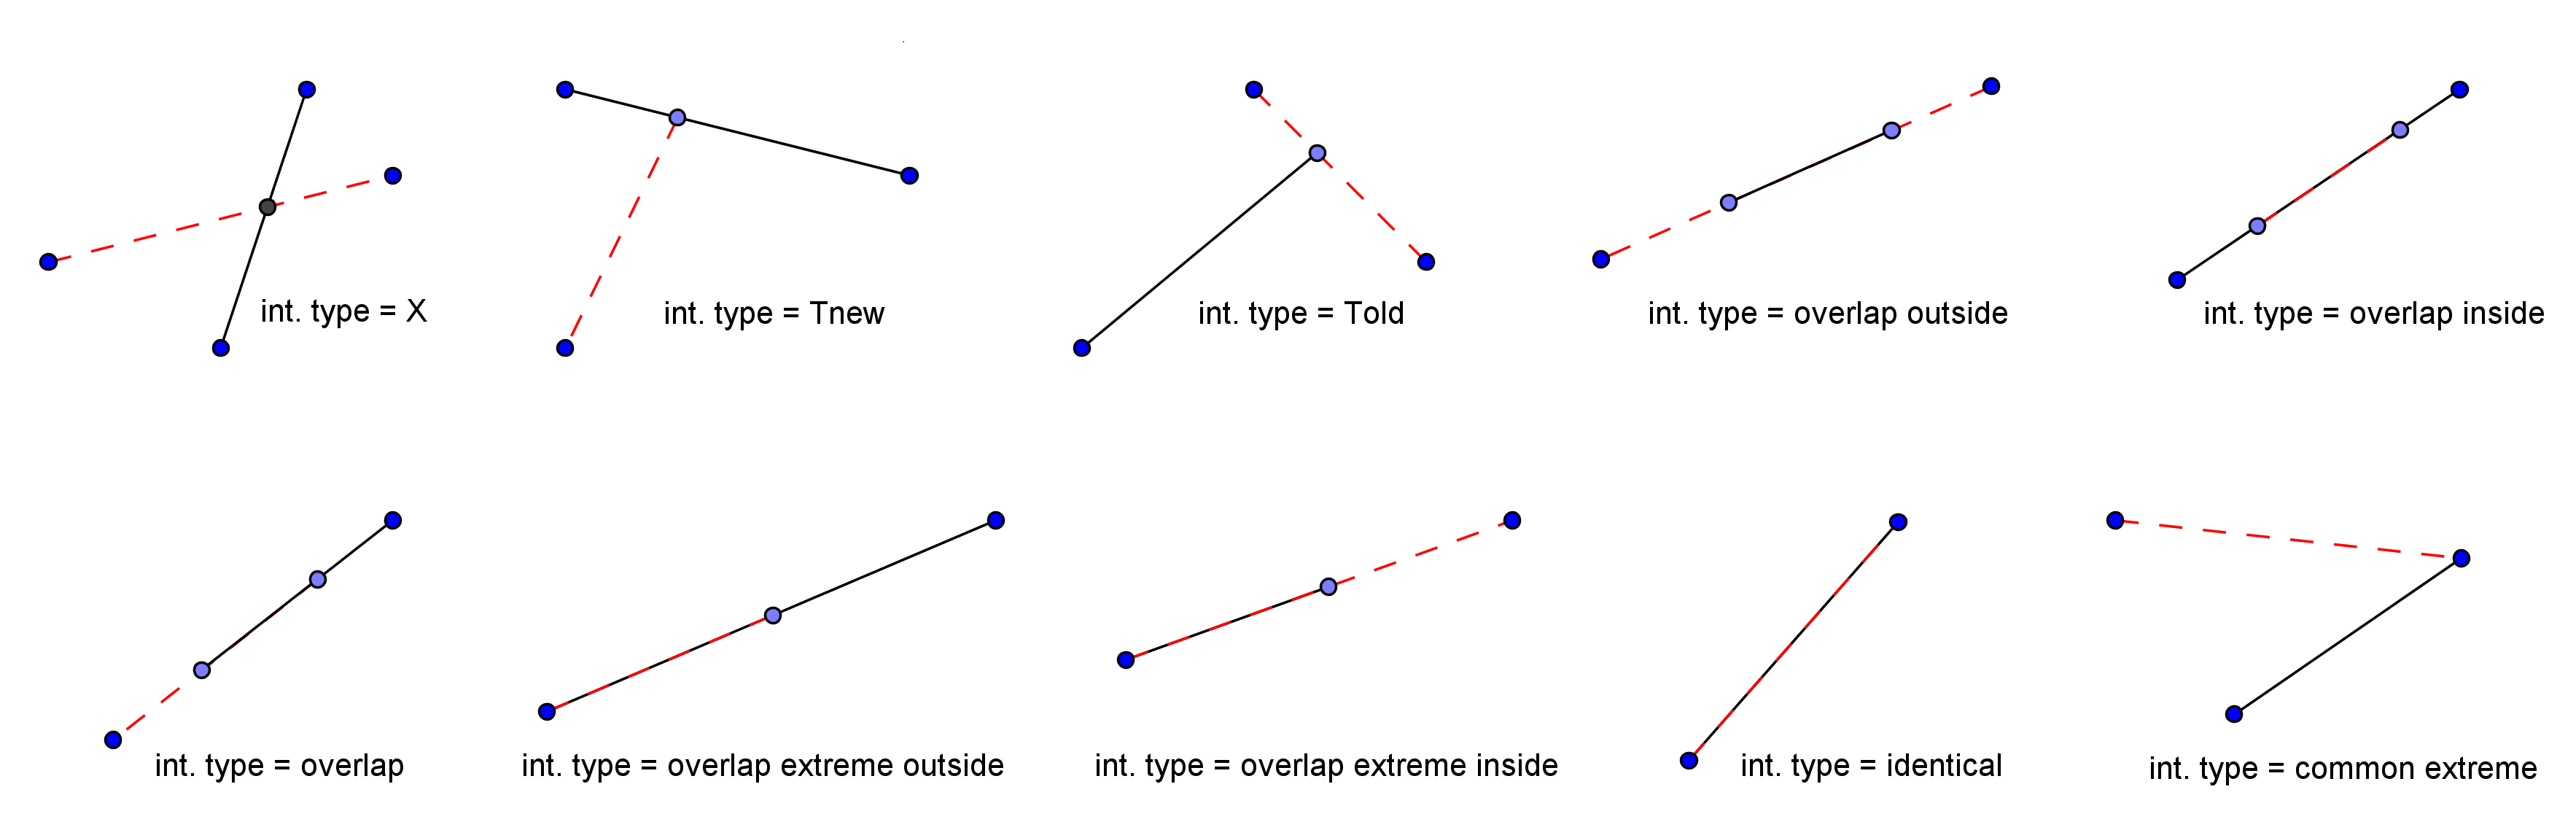
\includegraphics[width=1\textwidth]{int_type}
			\caption{Intersection types. In black the edge already in the graph, in red the new one.}
			\label{fig:frac_int_type}
		\end{figure}
		\subsubsection{The algorithm}
		Here we illustrate, through pseudocode and then with a detailed description, how the function \texttt{create\textunderscore graph} works.
		\begin{lstlisting}
		while(!eof){
			fracture = getline()
			create fracture edge_property 
			int_vect.clear()
			for e in edges(G){
				compute_intersection(e, fracture)
				if intersection exists{
					create Int_Layer with intersection information
					int_vect.push_back(Int_Layer)
				}	
			}
			if int_vect.empty(){
				add_edge to graph with fracture edge properties
			}
			else{
				reorder int_vect
				remove_duplicates inside int_vect
				refine_graph(fracture, int_vect)  
			}
		}		
		
		\end{lstlisting}
		The file is read fracture by fracture: for each of them the physical properties are stored in the edge\textunderscore property struct and the line number is used as identifier; a vertex descriptor called SRC is associated to the first extremity of the fracture, another called TGT to the second one. These vertex descriptors can be either associated to already existing vertices in case of same coordinates or to new ones otherwise. After the initialization part, we loop over the edges in the graph: for each of them the function \texttt{compute\textunderscore intersection} checks for intersections with the current fracture; if so, the corresponding \texttt{Int\textunderscore Layer} struct is created and pushed back in a vector which, by the end of the loop, will therefore contain all the intersections with the fracture we are currently reading. \\
		Once the loop over the edges is completed, if the intersection vector is empty, a new edge is created between SRC and TGT and the edge\textunderscore property is bundled to it, otherwise the vector is first reordered and then some "duplicates" are removed.
		The reordering phase consists exactly in ordering the vector from the nearest to the source to the farthest one; also the two intersections contained in the same struct (in those cases in which the intersection is a segment and not a single point) are reordered according to the same criterion (and if they are swapped the boolean variable \texttt{swapped} in the \texttt{Int\textunderscore layer} is switched from 0 to 1).
		The duplicates removal, performed by function \texttt{remove\textunderscore duplicates}, consists in keeping just one single struct among all of those related to the same intersection point; in \ref{fig:rem_dupl} an example is shown: 
		\begin{figure}
		\centering 
		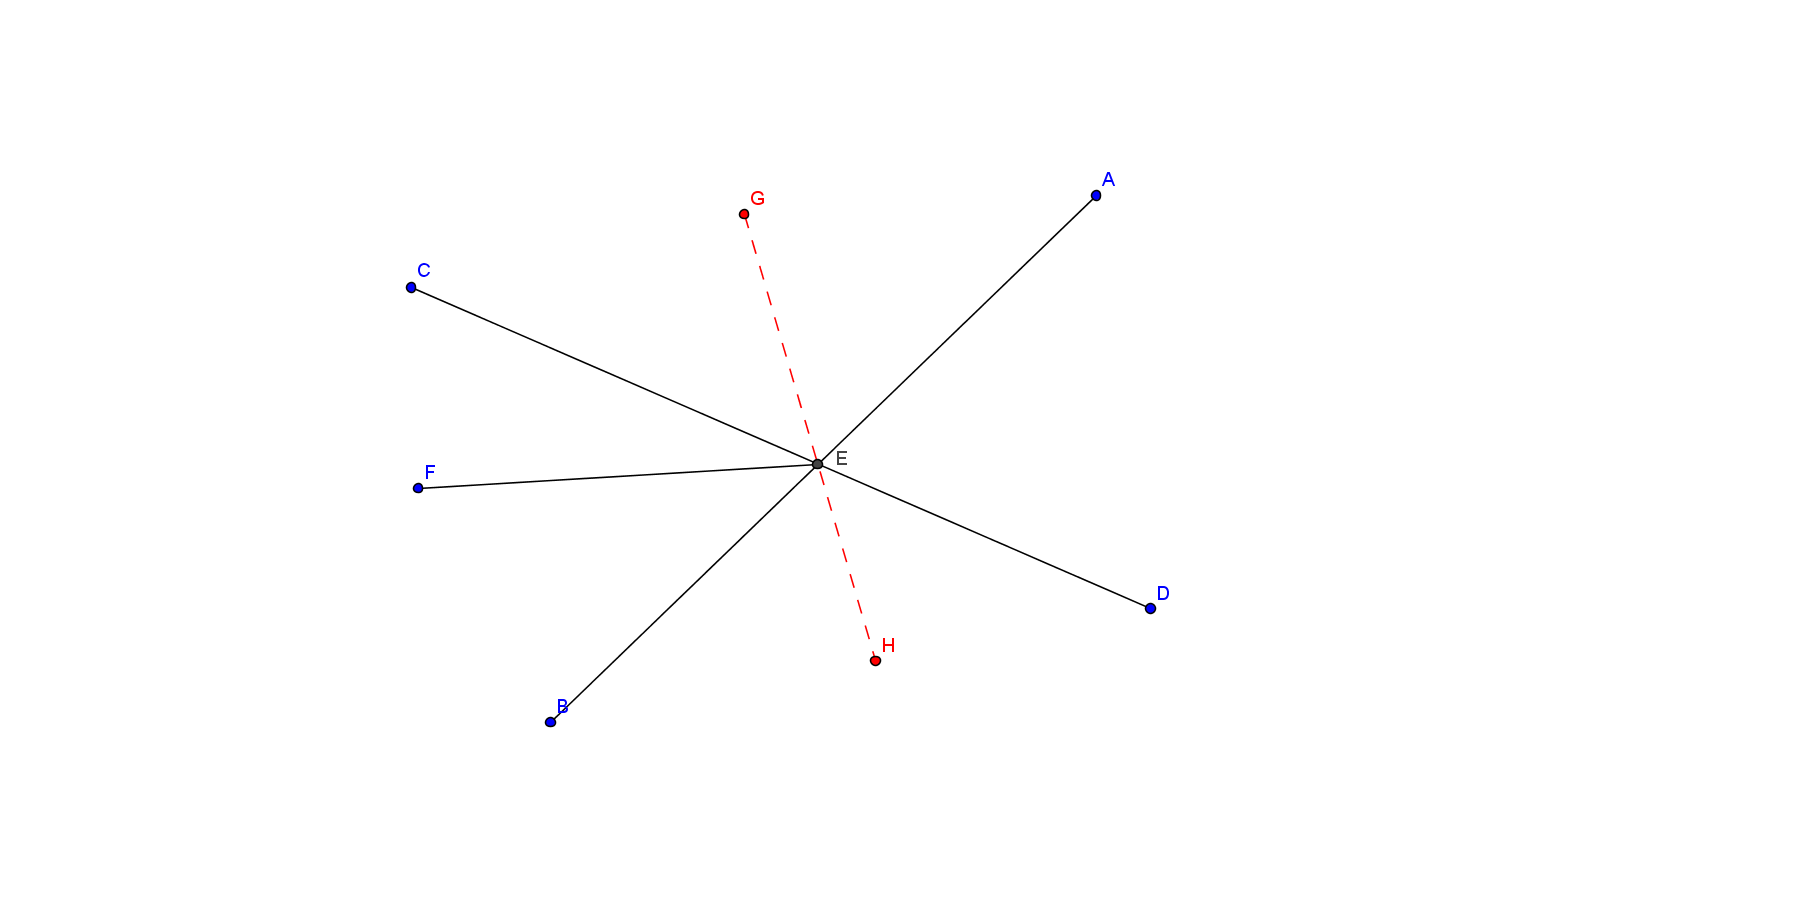
\includegraphics[width=1\textwidth]{rem_dupl}
		\caption{Example on duplicates removal}
		\label{fig:rem_dupl}
		\end{figure}
		before adding the new fracture (the red one), the graph has 5 edges and 6 vertices. Looping on the edges, the algorithm correctly detects one intersection with each edge, but there is only one intersection point, E, and no edge has to be modified by the insertion of the new fracture, therefore all the "duplicates" are discarded but one. Note that this happens just in case of multiple intersections of type "Told" or "common extreme". \\
		Now the vector is ready to be processed. We start passing to the function \texttt{refine\textunderscore graph} SRC and the first struct of the vector: this function performs different actions depending on the intersection type; the common goal is to resolve all the changes due to the insertion of the new fracture and related to that specific segment. The function returns as output the vertex descriptor which will be passed as source at the next iteration together with the second struct in the vector. This procedure goes on until the end of the intersection vector is reached; at the end, the vertex descriptor returned by the last call to \texttt{refine\textunderscore graph} is connected to TGT. \\
		In case of partial or total overlapping between the new fracture and an existing edge, a conflict between the corresponding edge properties happens: it is up to the user to decide how to solve it, and this is possible passing as optional parameter to \texttt{create\textunderscore graph} a lambda function \texttt{update\textunderscore edge\textunderscore properties} which will be used inside \texttt{refine\textunderscore graph} to merge old and new properties. The default behaviour is simply to keep the old property, totally discarding the new one.
		
		\subsubsection{A simple example}
		This example refers to \ref{fig:example_algo} and it aims at illustrating how the algorithm works.
		\begin{figure}
			\centering 
			\includegraphics[width=1\textwidth]{example_algo}
			\caption{Fracture in red is going to be added to the graph}
			\label{fig:example_algo}
		\end{figure}
		We consider the insertion of the fifth fracture (e): the previous four (a,b,c,d) have been already added and the graph they created is made of 8 vertices and 6 edges (AE, BE, CE, DE, FE, GH).  
		Since the extremities of the new fracture have coordinates different from all the other existing points, two new vertices I and J are created. Looping over the edges in the graph, we obtain a vector of six intersection structs; we reorder it and we remove four duplicates in point E.  (see table \ref{tab:table1}).
		Now we are left with a vector of two components: first of all we pass to refine\textunderscore graph the vertex descriptor I (which is the source of the new fracture) and the first intersection struct (related to point E); being the intersection of type T\textunderscore old, this function simply adds an edge between I and E and returns as next source E. At the second step, refine\textunderscore graph takes as input the current source (i.e. the output of the previous call to the function, i.e. E in this example) and the second intersection struct: in case of overlap\textunderscore outside the source is connected to the first intersection (EH), the properties of the old edge (HG) are updated and the second intersection is connected with the target (GJ). In conclusion, the insertion of this new fracture led to the creation of three new edges (all labelled with letter e in order to keep track of the fact they all part of the fifth fracture) and to the property updating of an existing one.
		
		\begin{table}[ht]
		\centering
		\caption{Simplified representation of the intersection vector}
		\label{tab:table1}
			\begin{tabular}[t]{ccc}
			\toprule
			Int. edge & Type & Int. point(s)\\
			\midrule
			AE & T\textunderscore old & E\\
			BE & T\textunderscore old & E\\
			FE & T\textunderscore old & E\\
			GH & overlap\textunderscore outside & \textbf{G and H}\\ 
			DE & T\textunderscore old & E\\		
			CE & T\textunderscore old & E\\
			\bottomrule
			\end{tabular} 
			\hfill
			\begin{tabular}[t]{ccc}
			\toprule
			Int. edge & Type & Int. point(s)\\
			\midrule
			AE & T\textunderscore old & E\\
			BE & T\textunderscore old & E\\
			FE & T\textunderscore old & E\\
			DE & T\textunderscore old & E\\		
			CE & T\textunderscore old & E\\
			GH & overlap\textunderscore outside & \textbf{H and G}\\ 
			\bottomrule
			\end{tabular} 
			\hfill
			\begin{tabular}[t]{ccc}
			\toprule
			Int. edge & Type & Int. point(s)\\
			\midrule
			AE & T\textunderscore old & E\\
			GH & overlap\textunderscore outside & G and H\\ 
			\bottomrule
			\end{tabular}
		\end{table}
	
	\subsubsection{A more complex example}
		In file \texttt{test\_all\_int\_cases.txt} we put a list of fractures with no property associated: the main goal of this example is to show that the code performs correctly whatever is the intersection type it has to handle. Indeed, the sequence of fractures is built in such a way that almost every intersection type appears during the construction of the graph. 
				\begin{figure}
					\centering 
					\includegraphics[width=1\textwidth]{graph_building_process}
					\caption{Fracture in red is going to be added to the graph}
					\label{fig:graph_steps}
				\end{figure}
		In figure \ref{graph_steps} we show how the graph is built step by step, one fracture at a time.
		



	\subsection{Diffusion on a vascular network}
%		\subsubsection{The problem}
	Ih this application we model and solve a diffusion problem on a vascular network, taking advantage also of the GetFem++ library, which is specifically built to solve FEM problems. \newline
	The diffusion problem is simply
	\begin{equation*}
		\left\{
		\begin{aligned}
		\Delta u = f \\
		u = 0 
		\end{aligned}
		\right.
	\end{equation*}
	with boundary conditions .... 	\newline
	The vascular network we use in the application is a prototype for a network with a sequence of bifurcations. There is a first single edge, that is the inflow one, that bifurcates in a Y on the plane (z?), then each extreme of this first bifurcation bifurcates again, but this time along the (x?) plane, then the four ends with which we end up bifurcate again on the (z?) plane, and so on . The algorithm can go on iteratively to any order of bifurcation, building a network that will be always contained in a unitary cube. We also considered randomization on the final coordinates of each end point, but the first two (i.e. the first edge will always be in the same position). We perform this random effect by taking a draw from a uniform distribution on [-1,1], and then recaling this draw with the scale parameter $re$, that stands for 'random effect'. We provide with the application a matlab script that generates such a network, given the desired number of orders of bifurcations and the entity(???) of the random effect.
		
	%Computational issues?? Complexity and time efficiency?

\end{document}
